\documentclass{beamer-control}
\usepackage{beamer-control-singlefile}
\INCLUDEONLY{The Loop Transfer Function}
\begin{document}
\CONCEPT{The Loop Transfer Function}

\begin{SUMMARY}
\begin{itemize}
\item Loop analysis
\item Calculating the loop transfer function
\end{itemize}
\vfill References:
\begin{itemize}
\item \astrom{§10.1}
\end{itemize}
\end{SUMMARY}



\SUBCONCEPT{Loop analysis}

\begin{frame}{Frequency in feedback}
\begin{itemize}
\item How may we assess the behaviour of a closed loop system by studying the open loop system properties?
\item Using transfer functions we can follow how a sinusoidal signal at a given frequency behaves in the feedback loop
\item We can then assess stability of the closed loop by noticing if this signal grows or decays - if it grows, we have an unstable system
\end{itemize}
\end{frame}

\begin{frame}{Loop transfer function}
Rather than calculating the characteristic polynomial of the closed loop system (which is limited in aiding design of a controller), we may instead analyse the \textit{loop transfer function}
\[L(s)=P(s)C(s)\]
which represents the transfer function from input at A to output at B multiplied by $-1$ (to account for negative feedback).

\begin{figure}
	\centering
	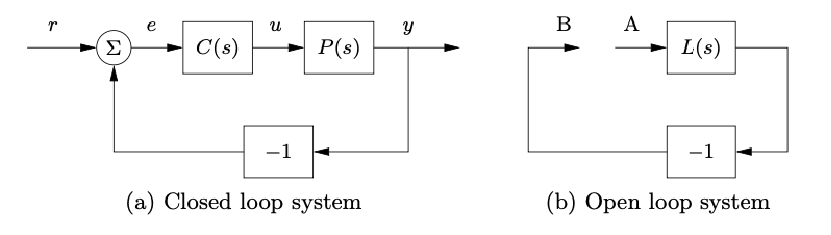
\includegraphics[width=\linewidth]{figure10.1}
	\\
	\textbf{Figure 10.1:} The loop transfer function.
\end{figure}
\end{frame}

\begin{frame}{Condition for stability}
	
\begin{itemize}
	\item Consider inputting a sinusoidal input of frequency $\omega_0$ at A
	\item To maintain the oscillation, the signal at B will also be a sinusoid with frequency $\omega_0$ and therefore
	\[L(i\omega_0)=-1.\]
	\item This condition says that our frequency response passes through the value of $-1$, known as the \textit{critical point}
	\item If we require stability at a frequency $\omega_c$ such that $\angle L\left(i \omega_{\mathrm{c}}\right)=180^{\circ}$, we therefore want our signal at B to have a smaller amplitude than the input at A and so $|L(i\omega_c)|<1$
\end{itemize}
\end{frame}


\SUBCONCEPT{Calculating the loop transfer function}

\begin{frame}{Example}
\begin{itemize}
\item Consider an electric motor with inertia $J$ and damping $c$ with proportional feedback controller and small delay in measurement of the motor position
\item The process dynamics are 
\[P(s) = \frac{k_I}{Js^2+cs}\]
\item The controller is of the form
\[C(s) = k_p\]
\item Therefore the loop transfer function (with added delay $\tau$) is 
\[L(s) = P(s) C(s) e^{-\tau s} = \frac{k_Ik_p}{Js^2+cs}e^{-\tau s}\]
\end{itemize}
\end{frame}

\begin{frame}{Example continued}
\begin{itemize}
\item The magnitude of the transfer function does not change with the delay but the phase does
\item Therefore we may get oscillations in the closed loop system if delay is present
\item We can use the Bode plots of the loop transfer function to assess what the magnitude of the output signal of the loop transfer function is corresponding to a phase of $180^\circ$
\item If $\theta_0$ is the phase of the undelayed system at a frequency $\omega_0$, then a time delay of 
\[\tau_c=\frac{\pi+\theta_0}{\omega_0}\]
will cause $L(i\omega_0)$ to be equal to $-1$
\end{itemize}
\end{frame}


\begin{frame}{Example continued}
\begin{itemize}
\item For no delay $\tau=0$, the phase of $L(s)$ approaches \ang{180} but doesn't reach it and so the system is stable
\item For a delay of $\tau=\tau_c$, when the phase of $L(s)$ is \ang{180}, the magnitude is $1$ and so the system maintains oscillation
\item For a delay of $\tau=3\tau_c$, the corresponding magnitude at \ang{180} phase is greater than $1$, resulting in instability
\end{itemize}
\begin{figure}
\centering
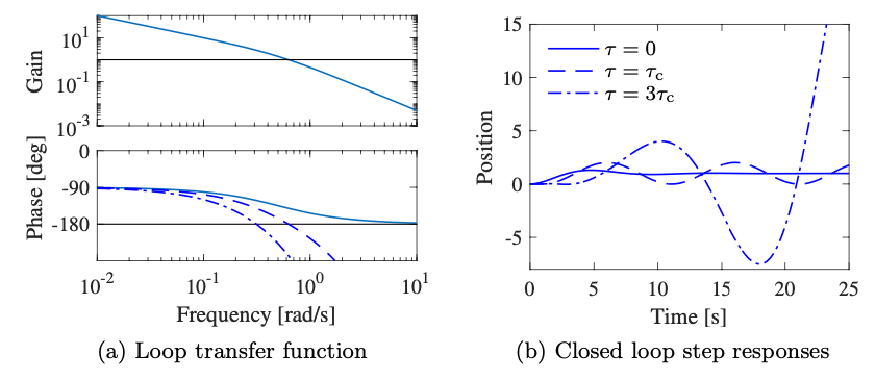
\includegraphics[width=0.8\linewidth]{figure10.3}
\\
\textbf{Figure 10.3:} The loop transfer function and step response for electric motor control system.
\end{figure}

\end{frame}


\SUMMARYFRAME
\FINALE

\end{document}
